\documentclass[../../main.tex]{subfiles}
\begin{document}

{\bf [解答]}

\subparagraph{(1)}

% TODO: 状況を説明する図
\begin{figure}[htb]
  \centering
  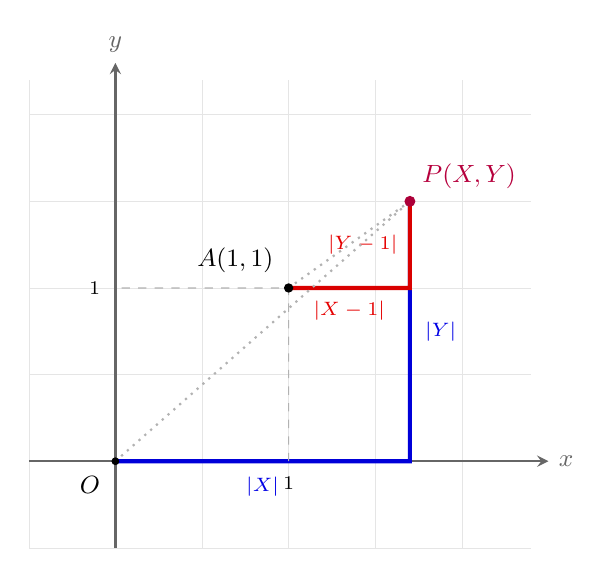
\begin{tikzpicture}[scale=2.2, >=stealth, every node/.style={font=\small}]

    % --- 1. 背景のグリッド（マンハッタン距離のイメージ）---
    \draw[help lines, gray!20, step=0.5] (-0.5, -0.5) grid (2.4, 2.2);

    % --- 2. 座標軸 ---
    \draw[->, thick, gray!80!black] (-0.5, 0) -- (2.5, 0) node[right] {$x$};
    \draw[->, thick, gray!80!black] (0, -0.5) -- (0, 2.3) node[above] {$y$};
    \node[below left=2pt] at (0, 0) {$O$};

    % --- 3. 基準点 O, A および動点 P の設定 ---
    % O(0,0), A(1,1), P(1.7, 1.5) の例
    \coordinate (O) at (0, 0);
    \coordinate (A) at (1.0, 1.0);
    \coordinate (P) at (1.7, 1.5);

    % --- 4. 点 O から点 P への距離 d(O,P) の経路 ---
    % 水平変位 |X| と垂直変位 |Y| (青色)
    \draw[line width=1.5pt, blue!85!black] (O) -- (1.7, 0) -- (P);
    \node[below=2pt, font=\scriptsize, blue!90!black] at (0.85, 0) {$|X|$};
    \node[right=2pt, font=\scriptsize, blue!90!black] at (1.7, 0.75) {$|Y|$};

    % --- 5. 点 A から点 P への距離 d(A,P) の経路 ---
    % 水平変位 |X-1| と垂直変位 |Y-1| (赤色)
    \draw[line width=1.5pt, red!85!black] (A) -- (1.7, 1.0) -- (P);
    \node[below=1pt, font=\scriptsize, red!90!black] at (1.35, 1.0) {$|X-1|$};
    \node[left=1pt, font=\scriptsize, red!90!black]  at (1.7, 1.25) {$|Y-1|$};

    % 直線距離（参考の点線）
    \draw[dotted, gray!60, thick] (O) -- (P);
    \draw[dotted, gray!60, thick] (A) -- (P);

    % --- 6. 基準点 A(1,1) の座標投影破線 ---
    \draw[dashed, gray!60] (1.0, 0) -- (A) -- (0, 1.0);
    \node[below=2pt, font=\scriptsize] at (1.0, 0) {$1$};
    \node[left=2pt, font=\scriptsize]  at (0, 1.0) {$1$};

    % --- 7. 主要点のプロットとラベル ---
    \node[circle, fill, inner sep=1.0pt] at (O) {};
    \node[circle, fill, inner sep=1.2pt] at (A) {}; \node[above left=2pt] at (A) {$A(1, 1)$};
    \node[circle, fill=purple!90!black, inner sep=1.4pt] at (P) {}; \node[above right=1pt, purple!95!black] at (P) {$P(X, Y)$};

  \end{tikzpicture}
  \caption{原点 $O(0,0)$，点 $A(1,1)$ と動点 $P(X,Y)$ の間の距離 $d(O,P), d(A,P)$ の状況}
  \label{fig:l1_distance_setup}
\end{figure}

一般に2点$S(x_1,y_1)$，$T(x_2,y_2)$に対し，
\begin{align}
  d(S,T)=|x_1-x_2|+|y_1-y_2| \label{eq:1}
\end{align}
である．
そこで$P(X,Y)$とおくと，
\begin{align}
  d(O,P)=|X|+|Y|，\qquad d(A,P)=|X-1|+|Y-1| \label{eq:2}
\end{align}
である．よって題意の条件は
\begin{align}
  d(O,P) = d(A,P) \iff |X|-|X-1| = -|Y|+|Y-1|
\end{align}
だから$f(t)=|t|-|t-1|$とおけば
\begin{align}
  f(x)+f(y)=0 \label{eq:3}
\end{align}
である．$f(t)$の具体的な関数形は
\begin{align}
  f(t)=
  \begin{cases}
    -1 & (t\le0)，\\
    2t-1 & (0\le t\le1)，\\
    1 & (1\le t)
  \end{cases}
\end{align}
だから$f(t)$のグラフは下図のようになる．

\begin{figure}[htb]
  \centering
  \begin{tikzpicture}[scale=1.8, >=stealth, every node/.style={font=\small}]

    % --- 1. 座標定義 ---
    \coordinate (O)     at (0, 0);
    \coordinate (P_neg) at (0, -1.0);       % 屈折点 (0, -1)
    \coordinate (P_mid) at (0.5, 0);        % 対称中心 (1/2, 0)
    \coordinate (P_pos) at (1.0, 1.0);       % 屈折点 (1, 1)

    % --- 2. 座標軸 ---
    \draw[->, thick, gray!80!black] (-1.4, 0) -- (2.5, 0) node[right] {$t$};
    \draw[->, thick, gray!80!black] (0, -1.5) -- (0, 1.6) node[above] {$f(t)$};
    \node[below left=2pt] at (O) {$O$};

    % --- 3. グラフ y = f(t) の描画 ---
    % (i) t <= 0: y = -1
    \draw[line width=1.8pt, blue!85!black] (-1.3, -1.0) -- (P_neg);
    % (ii) 0 <= t <= 1: y = 2t - 1
    \draw[line width=1.8pt, blue!85!black] (P_neg) -- (P_pos);
    % (iii) t >= 1: y = 1
    \draw[line width=1.8pt, blue!85!black] (P_pos) -- (2.3, 1.0);

    % --- 4. 投影破線と補助線 ---
    % 屈折点 (1, 1) からの投影
    \draw[dashed, gray!60] (0, 1.0) -- (P_pos) -- (1.0, 0);
    % 屈折点 (0, -1) の目盛り線
    \draw[dashed, gray!60] (P_neg) -- (-0.1, -1.0);

    % --- 5. 目盛りラベル ---
    \node[left=2pt, font=\scriptsize]  at (0, 1.0) {$1$};
    \node[left=2pt, font=\scriptsize]  at (0, -1.0) {$-1$};
    \node[below=2pt, font=\scriptsize] at (1.0, 0) {$1$};
    \node[below=2pt, font=\scriptsize, teal!90!black] at (P_mid) {$\frac{1}{2}$};

    % --- 6. 特徴点のプロット ---
    \node[circle, fill=blue!85!black, inner sep=1.2pt] at (P_neg) {};
    \node[circle, fill=blue!85!black, inner sep=1.2pt] at (P_pos) {};
    % 対称中心 (1/2, 0)
    \node[circle, fill=red!85!black, inner sep=1.4pt] at (P_mid) {};
    \node[above left=1pt, font=\scriptsize, red!90!black] at (P_mid) {対称中心};

    % --- 7. 各区間の数式ラベル ---
    \node[blue!90!black, font=\scriptsize, below] at (-0.7, -1.0) {$f(t) = -1$};
    \node[blue!90!black, font=\scriptsize, above left] at (0.45, 0.25) {$2t-1$};
    \node[blue!90!black, font=\scriptsize, above] at (1.7, 1.0) {$f(t) = 1$};

  \end{tikzpicture}
  \caption{関数 $f(t) = |t| - |t-1|$ のグラフ}
  \label{fig:ft_symmetric_graph}
\end{figure}

このグラフは$x=\dfrac{1}{2}$を軸に点対称だから\cref{eq:3}の条件は
\begin{itemize}
  \item $X\ge1\ \text{かつ}\ Y\le0$ \\
  \item $X\le0\ \text{かつ}\ Y\ge1$ \\
  \item $X+Y=1$
\end{itemize}
となる．これを図示すると下図の斜線部（境界含む）となる．

\begin{figure}[htb]
  \centering
  \begin{tikzpicture}[scale=1.9, >=stealth, every node/.style={font=\small}]

    % --- 1. 座標定義 ---
    \coordinate (O)    at (0, 0);
    \coordinate (P_01) at (0, 1.0);  % (0, 1)
    \coordinate (P_10) at (1.0, 0);  % (1, 0)

    % --- 2. 求める領域（斜線部、境界含む）のハッチング塗りつぶし ---
    % (i) X <= 0 かつ Y >= 1 の半無限帯状領域 (表示範囲 x in [-1.4, 0], y in [1, 2.4])
    \fill[pattern=north east lines, pattern color=blue!65, opacity=0.8]
    (-1.4, 1.0) rectangle (0, 2.4);

    % (ii) X >= 1 かつ Y <= 0 の半無限帯状領域 (表示範囲 x in [1, 2.4], y in [-1.4, 0])
    \fill[pattern=north east lines, pattern color=blue!65, opacity=0.8]
    (1.0, -1.4) rectangle (2.4, 0);

    % --- 3. 領域の境界線および線分 X + Y = 1 ---
    % 中央の線分 X + Y = 1 (0 <= X <= 1)
    \draw[line width=2.0pt, blue!85!black] (P_01) -- (P_10);

    % 第2象限側の境界線 (X <= 0, Y = 1 および X = 0, Y >= 1)
    \draw[line width=2.0pt, blue!85!black] (-1.4, 1.0) -- (P_01);
    \draw[line width=2.0pt, blue!85!black] (P_01) -- (0, 2.4);

    % 第4象限側の境界線 (X = 1, Y <= 0 および X >= 1, Y = 0)
    \draw[line width=2.0pt, blue!85!black] (1.0, -1.4) -- (P_10);
    \draw[line width=2.0pt, blue!85!black] (P_10) -- (2.4, 0);

    % 直線 X + Y = 1 の延長線（参考破線）
    \draw[dashed, blue!40, thick] (-1.3, 2.3) -- (P_01);
    \draw[dashed, blue!40, thick] (P_10) -- (2.3, -1.3);

    % --- 4. 座標軸 ---
    \draw[->, thick, gray!80!black] (-1.6, 0) -- (2.7, 0) node[right] {$x$};
    \draw[->, thick, gray!80!black] (0, -1.6) -- (0, 2.7) node[above] {$y$};
    \node[below left=2pt] at (O) {$O$};

    % --- 5. 目盛りと主要屈折点のプロット ---
    \node[circle, fill=blue!90!black, inner sep=1.5pt] at (P_01) {};
    \node[circle, fill=blue!90!black, inner sep=1.5pt] at (P_10) {};

    \node[left=3pt, font=\scriptsize]  at (0, 1.0) {$1$};
    \node[below=3pt, font=\scriptsize] at (1.0, 0) {$1$};

    % 基準点 A(1, 1) のプロット（参考）
    \draw[dotted, gray!60] (1.0, 0) -- (1.0, 1.0) -- (0, 1.0);
    \node[circle, fill=gray!70, inner sep=1.2pt] at (1.0, 1.0) {};
    \node[above right=1pt, font=\scriptsize, gray!80!black] at (1.0, 1.0) {$A(1,1)$};

    % 直線ラベル
    \node[blue!90!black, font=\footnotesize\bfseries, above right] at (0.6, 0.4) {$x + y = 1$};

    % 各領域の補助ラベル
    \node[blue!90!black, font=\scriptsize, align=center] at (-0.7, 1.7)
    {$x \le 0$\\[1pt]$y \ge 1$};
    \node[blue!90!black, font=\scriptsize, align=center] at (1.7, -0.7)
    {$x \ge 1$\\[1pt]$y \le 0$};

  \end{tikzpicture}
  \caption{(1) における点 $P$ の存在範囲（斜線部および境界線）}
  \label{fig:p_region_part1}
\end{figure}

\subparagraph{(2)}

(1)と同様$P(X,Y)$とおく．$Q(a,a^2-1)$だから
\begin{align}
  \begin{cases}
    d(O,P) = |X| + |Y| \\
    d(P,Q) = |X-a| + |Y-a^2-1|
  \end{cases}
\end{align}
であり，題意の条件$d(O,P)=d(P,Q)$は
\begin{align}
  |X-a|+|Y-a^2-1|=|X|+|Y| \label{eq:4}
\end{align}
である．
よってこれを満たす$a\ge 0$が存在するような$(X,Y)$を求めれば良い．
絶対値を外す場合分けは
\begin{align}
  \begin{cases}
    X \le 0, 0 \le X \le a, a \le X \\
    Y \le 0, 0 \le Y \le a^2+1, a^2+1 \le Y
  \end{cases}
\end{align}
で合計$3\times 3=9$通りである．
また
\begin{align}
  (a^2+1)-a=\left(a-\dfrac{1}{2}\right)^2+\dfrac{3}{4}>0
\end{align}
より$a^2+1>a$である．

\begin{figure}[htb]
  \centering
  \begin{tikzpicture}[scale=2.2, >=stealth, every node/.style={font=\small}]

    % --- 1. 定数・パラメータ設定 (a > 0, 例として a = 1.2, a^2+1 = 2.44) ---
    \def\aVal{1.2}
    \pgfmathsetmacro{\yTop}{\aVal*\aVal + 1.0} % 2.44

    \coordinate (O)     at (0, 0);
    \coordinate (X_a)   at (\aVal, 0);
    \coordinate (Y_top) at (0, \yTop);
    \coordinate (Q)     at (\aVal, \yTop);

    % --- 2. 9分割領域の彩色 ---
    % 有効な 3 領域 (0 <= Y <= a^2+1) の薄い塗りつぶし
    % (ア) X <= 0, 0 <= Y <= a^2+1
    \fill[teal!12, opacity=0.8] (-1.0, 0) rectangle (0, \yTop);
    % (イ) 0 <= X <= a, 0 <= Y <= a^2+1 (中央長方形)
    \fill[blue!15, opacity=0.8] (0, 0) rectangle (\aVal, \yTop);
    % (ウ) X >= a, 0 <= Y <= a^2+1
    \fill[orange!12, opacity=0.8] (\aVal, 0) rectangle (2.2, \yTop);

    % 四隅および上下の不適領域 (薄いグレー)
    \fill[gray!8, opacity=0.7] (-1.0, \yTop) rectangle (2.2, 3.1);
    \fill[gray!8, opacity=0.7] (-1.0, -0.8) rectangle (2.2, 0);

    % --- 3. 座標軸 ---
    \draw[->, thick, gray!80!black] (-1.1, 0) -- (2.4, 0) node[right] {$X$};
    \draw[->, thick, gray!80!black] (0, -0.9) -- (0, 3.2) node[above] {$Y$};
    \node[below left=2pt] at (O) {$O$};

    % --- 4. 境界直線群 (X = a, Y = a^2+1) ---
    % 垂直境界 X = a
    \draw[thick, dashed, blue!85!black] (\aVal, -0.8) -- (\aVal, 3.1);
    \node[blue!90!black, font=\scriptsize, above] at (\aVal, 3.1) {$X = a$};
    \node[below=2pt, font=\scriptsize, blue!90!black] at (\aVal, 0) {$a$};

    % 水平境界 Y = a^2 + 1
    \draw[thick, dashed, red!85!black] (-1.0, \yTop) -- (2.2, \yTop);
    \node[red!90!black, font=\scriptsize, right] at (2.2, \yTop) {$Y = a^2+1$};
    \node[left=2pt, font=\scriptsize, red!90!black] at (0, \yTop) {$a^2+1$};

    % --- 5. 点 Q(a, a^2+1) のプロット ---
    \node[circle, fill=red!85!black, inner sep=1.2pt] at (Q) {};
    \node[above right=1pt, font=\footnotesize, red!90!black] at (Q) {$Q(a, a^2+1)$};

    % --- 6. 各領域のラベル (表の分類に対応) ---
    % 注目する中央帯 (0 <= Y <= a^2+1)
    \node[font=\footnotesize\bfseries, teal!90!black, align=center] at (-0.5, 1.2) {(ア)\\$X \le 0$};
    \node[font=\footnotesize\bfseries, blue!90!black, align=center] at (0.6, 1.2) {(イ)\\$0 \le X \le a$};
    \node[font=\footnotesize\bfseries, orange!95!black, align=center] at (1.7, 1.2) {(ウ)\\$a \le X$};

    % 上段 (Y >= a^2+1, 不適)
    \node[font=\scriptsize, gray!60!black] at (-0.5, 2.75) {不適};
    \node[font=\scriptsize, gray!60!black] at (0.6, 2.75) {不適};
    \node[font=\scriptsize, gray!60!black] at (1.7, 2.75) {不適};

    % 下段 (Y <= 0, 不適)
    \node[font=\scriptsize, gray!60!black] at (-0.5, -0.45) {不適};
    \node[font=\scriptsize, gray!60!black] at (0.6, -0.45) {不適};
    \node[font=\scriptsize, gray!60!black] at (1.7, -0.45) {不適};

  \end{tikzpicture}
  \caption{絶対値の符号に応じた $(X,Y)$ 平面の 9 分割と検討対象領域（ア, イ, ウ）}
  \label{fig:xy_nine_regions_split}
\end{figure}

各場合における\cref{eq:4}を表にまとめると以下のようになる．

\begin{table}[htb]
  \centering
  \renewcommand{\arraystretch}{1.6}
  \begin{tabular}{c|c|c|c}
    & $X\le0$ & $0\le X\le a$ & $a\le X$ \\ \hline
    $Y\le0$ & $a^2+a+1=0$ (不適) & $2X=a^2+a+1$ (不適) & $a^2-a+1=0$ (不適) \\ \hline
    (ア) $0\le Y\le a^2+1$ & $2Y=a^2+a+1$ & (イ) $2(X+Y)=a^2+a+1$ & (ウ) $2Y=a^2-a+1$ \\ \hline
    $a^2+1\le Y$ & $a^2-a+1=0$ (不適) & $2X=-a^2+a-1$ (不適) & $a^2+a+1=0$ (不適)
  \end{tabular}
  \caption{点$P$の位置による場合分け}
\end{table}

各領域を順番に考える．
まず$a^2\pm a+1>0$より，表の四隅の場合を満たす$a\ge 0$は存在せず不適である．

また，$y\le0, a^2+1 \le y$，$0\le x\le a$の場合には
\begin{align}
  0\le \pm a^2+a \pm 1 \le 2a
\end{align}
が必要だがこれを満たす$a$も存在せず不適である．

以上より$0\le Y\le a^2+1$の場合だけを考えればよい．
この時の\cref{eq:4}を満たす$(X,Y)$は図示すると下図のようになる．
ここで$0 \le a$より
\begin{align}
  0 \le \dfrac{1}{2}\left(a^2-a+1\right) \le \dfrac{1}{2}\left(a^2+a+1\right) \le a^2+1
\end{align}
だから，$0\le Y\le a^2+1$の条件は常に満たされることに注意して以下各場合を考える．

% 0\le Y\le a^2+1の時の(X,Y)のグラフ
\begin{figure}[htb]
  \centering
  \begin{tikzpicture}[scale=2.2, >=stealth, every node/.style={font=\small}]

    % --- 1. 定数・座標パラメータ (例: a = 1.3) ---
    % Y_max = a^2 + 1 ≈ 2.69
    % Y_top = (a^2 + a + 1)/2 ≈ 1.995
    % Y_bot = (a^2 - a + 1)/2 ≈ 0.695
    \def\aVal{1.3}
    \pgfmathsetmacro{\yMax}{\aVal*\aVal + 1.0}
    \pgfmathsetmacro{\yTop}{(\aVal*\aVal + \aVal + 1.0) / 2.0}
    \pgfmathsetmacro{\yBot}{(\aVal*\aVal - \aVal + 1.0) / 2.0}

    \coordinate (O)     at (0, 0);
    \coordinate (P_top) at (0, \yTop);      % (0, (a^2+a+1)/2)
    \coordinate (P_bot) at (\aVal, \yBot);  % (a, (a^2-a+1)/2)

    % --- 2. 座標軸 (大文字 X, Y) ---
    \draw[->, thick, gray!80!black] (-1.4, 0) -- (2.6, 0) node[right] {$X$};
    \draw[->, thick, gray!80!black] (0, -0.3) -- (0, 3.1) node[above] {$Y$};
    \node[below left=2pt] at (O) {$O$};

    % --- 3. 領域上限の直線 Y = a^2 + 1 ---
    \draw[thick, dashed, teal!85!black] (-1.3, \yMax) -- (2.4, \yMax);
    \node[teal!90!black, font=\scriptsize, above right] at (1.5, \yMax) {$Y = a^2 + 1$};
    \node[left=2pt, font=\scriptsize, teal!90!black] at (0, \yMax) {$a^2 + 1$};
    \node[circle, fill=teal!85!black, inner sep=1.0pt] at (0, \yMax) {};

    % --- 4. グラフの描画（太線実線で連続接続）---
    % (ア) X <= 0: 水平線 Y = (a^2 + a + 1)/2
    \draw[line width=1.8pt, blue!85!black] (-1.3, \yTop) -- (P_top);

    % (イ) 0 <= X <= a: 傾き -1 の線分 X + Y = (a^2 + a + 1)/2
    \draw[line width=1.8pt, blue!85!black] (P_top) -- (P_bot);

    % (ウ) X >= a: 水平線 Y = (a^2 - a + 1)/2
    \draw[line width=1.8pt, blue!85!black] (P_bot) -- (2.4, \yBot);

    % 線分（イ）の X 軸への延長破線
    \draw[dashed, gray!45] (P_bot) -- ({\yTop}, 0);

    % --- 5. 投影破線と目盛り ---
    % X = a の破線
    \draw[dashed, gray!60] (\aVal, 0) -- (P_bot);
    \node[below=2pt, font=\scriptsize] at (\aVal, 0) {$a$};

    % Y = (a^2 - a + 1)/2 の破線
    \draw[dashed, gray!60] (0, \yBot) -- (P_bot);
    \node[left=2pt, font=\scriptsize] at (0, \yBot) {$\frac{1}{2}(a^2 - a + 1)$};

    % Y = (a^2 + a + 1)/2 のラベル
    \node[above right=1pt, font=\scriptsize] at (P_top) {$\frac{1}{2}(a^2 + a + 1)$};

    % --- 6. 屈折点のプロット ---
    \node[circle, fill=blue!90!black, inner sep=1.5pt] at (P_top) {};
    \node[circle, fill=blue!90!black, inner sep=1.5pt] at (P_bot) {};

    % --- 7. 各区間の丸付きラベル（ア, イ, ウ）---
    % (ア) のラベル
    \node[draw=black, circle, inner sep=1pt, font=\scriptsize, fill=white]
    (lbl_a) at (-0.7, \yTop + 0.35) {ア};
    \draw[->, thin, gray!70] (lbl_a) -- (-0.7, \yTop + 0.05);

    % (イ) のラベル
    \node[draw=black, circle, inner sep=1pt, font=\scriptsize, fill=white]
    (lbl_i) at (0.85, 1.6) {イ};
    \draw[->, thin, gray!70] (lbl_i) -- ($ (P_top)!0.4!(P_bot) + (0.05, 0.05) $);

    % (ウ) のラベル
    \node[draw=black, circle, inner sep=1pt, font=\scriptsize, fill=white]
    (lbl_u) at (1.85, \yBot + 0.35) {ウ};
    \draw[->, thin, gray!70] (lbl_u) -- (1.85, \yBot + 0.05);

  \end{tikzpicture}
  \caption{$0 \le Y \le a^2+1$ における各区間（ア, イ, ウ）の $(X, Y)$ の関係と上限 $Y = a^2+1$}
  \label{fig:xy_relation_for_fixed_a}
\end{figure}

\subparagraph{(ア) $x\le0$のとき}

前述のように$0 \le Y \le a^2+1$以外の条件を考えればよく，
この時，
\begin{align}
  Y
  &=\dfrac{a^2+a+1}{2} \\
  &=\dfrac{1}{2}\left(a+\dfrac{1}{2}\right)^2+\dfrac{3}{8} \\
  & \ge \dfrac{1}{2}
\end{align}
の範囲は
\begin{align}
  X\le0，\qquad Y\ge\dfrac{1}{2} \label{eq:5}
\end{align}
である．

\subparagraph{（イ）$0\le x\le a$のとき}

前述のように$0 \le Y \le a^2+1$以外の条件を考えればよく，
\begin{align}
  0 \le X \le a  \label{eq:6}
\end{align}
の元で
\begin{align}
  Y
  &=\dfrac{1}{2}a^2+\dfrac{1}{2}a+\dfrac{1}{2}-X\\
  &=\dfrac{1}{2}\left(a+\dfrac{1}{2}\right)^2+\dfrac{3}{8}-X \label{eq:7}
\end{align}
の右辺の値域を考えて
\begin{align}
  Y &\ge \dfrac{1}{2}\left(X+\dfrac{1}{2}\right)^2+\dfrac{3}{8}-X \\
  &= \dfrac{1}{2}\left(X-\dfrac{1}{2}\right)^2+\dfrac{3}{8} \quad (X \ge 0) \label{eq:8}
\end{align}
となる．

\subparagraph{(ウ) $a\le x$のとき}

前述のように$0 \le Y \le a^2+1$以外の条件を考えればよく，
$Y$の表式
\begin{align}
  Y = \dfrac{1}{2}\left(a-\dfrac{1}{2}\right)^2+\dfrac{3}{8}
\end{align}
の値域を$a \le X$で考えると
\begin{align}
  \begin{cases}
    Y \ge\dfrac{1}{2}\left(X-\dfrac{1}{2}\right)^2+\dfrac{3}{8}
    & \left(0\le x\le\dfrac{1}{2}\right)，\\
    Y \ge\dfrac{3}{8} & \left(\dfrac{1}{2}\le x\right)
  \end{cases} \label{eq:9}
\end{align}
である．
\casesend

以上\cref{eq:7,eq:8,eq:9}をまとめると，求める範囲は
\begin{align}
  \begin{cases}
    Y\ge\dfrac{1}{2} & (X\le0)，\\
    Y\ge\dfrac{1}{2}\left(X-\dfrac{1}{2}\right)^2+\dfrac{3}{8}
    & \left(0\le X\le\dfrac{1}{2}\right)，\\
    Y\ge\dfrac{3}{8} & \left(\dfrac{1}{2}\le X\right)
  \end{cases}
\end{align}
である．図示すると下図の斜線部となる（境界を含む）．

\begin{figure}[htb]
  \centering
  \begin{tikzpicture}[x=3cm,y=3cm,>=stealth,every node/.style={font=\small}]
    \fill[pattern=north east lines,pattern color=blue!60]
    (-0.7,1.25) -- (1.65,1.25) -- (1.65,0.375) -- (0.5,0.375)
    -- plot[domain=0.5:0,samples=60] (\x,{0.5*(\x-0.5)*(\x-0.5)+0.375})
    -- (-0.7,0.5) -- cycle;
    \draw[->,thick] (-0.8,0) -- (1.8,0) node[right] {$x$};
    \draw[->,thick] (0,-0.1) -- (0,1.4) node[above] {$y$};
    \draw[very thick,blue!85!black] (-0.7,0.5) -- (0,0.5);
    \draw[very thick,blue!85!black,domain=0:0.5,samples=60]
    plot (\x,{0.5*(\x-0.5)*(\x-0.5)+0.375});
    \draw[very thick,blue!85!black] (0.5,0.375) -- (1.65,0.375);
    \draw[dashed,gray!60] (0.5,0) -- (0.5,0.375) -- (0,0.375);
    \node[below left] at (0,0) {$O$};
    \node[above left] at (0,0.5) {$\frac{1}{2}$};
    \node[below left] at (0,0.375) {$\frac{3}{8}$};
    \node[below] at (0.5,0) {$\frac{1}{2}$};
    \node[fill=white,inner sep=3pt] at (0.95,0.95)
    {$y=\frac{1}{2}\left(x-\frac{1}{2}\right)^2+\frac{3}{8}$};
    \draw[->,gray!70] (0.7,0.82) -- (0.25,0.43);
  \end{tikzpicture}
  \caption{(2)の点$P$の範囲}
\end{figure}

\end{document}
